\documentclass[10pt]{exam}
\usepackage[hon]{template-for-exam}
\usepackage{graphicx}

\title{Sink the Boat Lab}
\author{Rohrbach}
\date{\today}

\begin{document}
\maketitle


\section*{The Problem}

You have survived a ship wreck somewhere in the Atlantic Ocean (\emph{i.e.} classroom floor). You swam to an isolated island (\emph{i.e.} your desk) and have lived happily for a few years. It is like paradise for you: plenty of food, pristine beaches, peace and quiet. You've really enjoyed your life and you do not want it changed. Suddenly a threat shows up at the horizon in the form of an enemy boat which approaches the island. You have somewhat anticipated this problem and constructed a type of pendulum which could shoot bombs (\emph{i.e.} metal/wooden spheres) at this enemy ship (\emph{i.e.} paper boat on the classroom floor). 

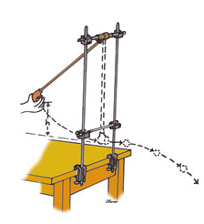
\includegraphics{release-your-potential.png}


The ship approaches and its crew has decided to take a lunch break (which will last most of our period) near the island before attacking you. During this time you are working hard at calculating the necessary setup (height) of the pendulum to make an attempt at defeating your enemy. You have only one shot available. Your life (\emph{i.e.} your grade) is at stake. Can you sink the boat?


\section*{Your Solution}

Initially, you should use the whiteboard to work out the problem with your group.  When you're ready, include a diagram of the setup and show your work below (or on a separate sheet of paper).  You will be taking a picture of your work and then explaining it in your lab report.

\pagebreak


\section*{Lab Report Guidelines}

\subsection*{Purpose:}  
Write a brief statement explaining the problem.  What are you trying to accomplish?


\subsection*{Procedure/Calculations:}
Take a picture with your phone of your calculations and insert them in the word document.  Your calculations should be \emph{well organized} and should include a labeled \emph{diagram} of the lab setup.  You should also include a paragraph explaining the mathematical steps you used to solve the problem 

\subsection*{Results:}
Write a few sentences explaining your results.  Did you achieve the objective?  Was there any obvious issues in completing the launch?

\subsection*{Conclusion/Discussion:}
Write a paragraph that addresses the following questions.

\begin{enumerate}
  \item Explain your results. Were you accurate?  Why or why not? 
  \item Explain what you learned during the experiment
  \item Explain where the errors came from.  Be specific—you should never use vague allusions to “human error.”  What could be done in the future to improve your results?
  \item Did you achieve the purpose of the lab?  Explain.
\end{enumerate}
	


\end{document}